
% ════════════════════════════════════════
% 模型检验与分析（06.模型检验.tex）
% ════════════════════════════════════════
\section{模型检验与分析}

为验证本文构建的模型的有效性和稳健性，进行以下检验。本文模型为线性规划优化模型，其最优性由求解器严格保证\cite{boyd2004}，因此检验重点在于约束满足程度、能量守恒精度与参数灵敏度。

\subsection{误差分析}

对问题一的最优解逐项核验其约束满足情况与能量守恒精度，结果如表\ref{tab:error}所示。

\begin{longtable}{>{\centering\arraybackslash}p{0.30\textwidth}>{\centering\arraybackslash}p{0.26\textwidth}>{\raggedright\arraybackslash}p{0.36\textwidth}}
  \caption{模型误差分析结果}
  \label{tab:error} \\
  \toprule
  检验项 & 检验结果 & 说明 \\
  \midrule
  \endfirsthead
  \caption{模型误差分析结果（续）} \\
  \toprule
  检验项 & 检验结果 & 说明 \\
  \midrule
  \endhead
  \bottomrule
  \endfoot
  功率平衡最大残差 & $1.36\times10^{-12}$ & 能量守恒严格满足 \\
  储电量越界次数 & 0 & 全程处于 $[1200,10800]$ kWh \\
  充放电功率越界次数 & 0 & 始终不超过 5000 kW \\
  储电初值约束 & 满足 & $E_0=6000$ kWh，与附录1给定一致 \\
  日循环约束残差 & 0 & $E_0=E_{144}=6000$ kWh \\
\end{longtable}

如表\ref{tab:error}所示，最优解的功率平衡残差处于 $10^{-12}$ 量级，储能荷电状态与充放电功率全程处于约束区间，日循环约束严格成立，验证了模型求解的正确性与数值精度。

\subsection{灵敏度分析}

为检验模型对关键参数的稳健性，分别调整储能充放电效率、最大充放电功率、储电量下限与负荷水平，观察全天购电费的变化，结果如表\ref{tab:sensitivity}所示。

\begin{longtable}{>{\centering\arraybackslash}p{0.30\textwidth}>{\centering\arraybackslash}p{0.30\textwidth}>{\raggedright\arraybackslash}p{0.32\textwidth}}
  \caption{灵敏度分析结果}
  \label{tab:sensitivity} \\
  \toprule
  参数变化 & 输出变化 & 灵敏度评估 \\
  \midrule
  \endfirsthead
  \caption{灵敏度分析结果（续）} \\
  \toprule
  参数变化 & 输出变化 & 灵敏度评估 \\
  \midrule
  \endhead
  \bottomrule
  \endfoot
  $\eta=0.85$ & 36603.41 元 & 费用上升 4.20\% \\
  $\eta=0.95$ & 33767.03 元 & 费用下降 3.87\% \\
  $P_{\max}=4000$ & 35247.87 元 & 费用上升 0.34\% \\
  $P_{\max}=6000$ & 35083.29 元 & 费用下降 0.12\% \\
  $E_{\min}=1500$ & 35329.91 元 & 费用上升 0.58\% \\
  负荷 $+5\%$ & 38834.17 元 & 费用上升 10.55\% \\
  负荷 $-5\%$ & 31552.18 元 & 费用下降 10.18\% \\
\end{longtable}

如表\ref{tab:sensitivity}所示，购电费对充放电效率最为敏感，效率每提高 5\% 可使费用下降约 4\%，说明储能效率是影响经济性的关键因素；充放电功率与储电量下限的小幅变化对费用的影响均不足 1\%，模型稳健；负荷水平按比例影响费用，符合能量平衡的线性规律。综上，在上述参数摄动范围内模型表现稳定。

\subsection{稳健性检验与适用边界}

误差分析与灵敏度分析表明，模型在给定数据下数值可靠，对储能参数的摄动也不敏感；但这两项检验都建立在同一套数据与同一比较基准之上，尚不足以说明结论是否依赖于特定数据样本、求解算法以及未加说明的建模前提。为此，本节从数据摄动、算法替换、预报展开口径、无储能对照与逐日收益方向五个角度补充检验，并明确模型的适用边界。

\textbf{1.数据摄动检验}

为检验结果是否依赖特定数据样本，对问题二全年 334 天的负荷与光伏数据施加乘性高斯噪声 $\varepsilon\sim N(0,\sigma^{2})$，即令 $\tilde{L}_{d,k}=L_{d,k}(1+\varepsilon_{d,k}^{L})$、$\tilde{S}_{d,k}=S_{d,k}(1+\varepsilon_{d,k}^{S})$，在噪声强度 $\sigma=5\%$ 与 $\sigma=10\%$ 下分别随机重复 6 次与 3 次，重新求解全年逐日滚动模型，统计 2 月 1 日—12 月 31 日购电费的分布，结果如表\ref{tab:robust}所示。

\begin{longtable}{>{\centering\arraybackslash}p{0.18\textwidth}>{\centering\arraybackslash}p{0.26\textwidth}>{\centering\arraybackslash}p{0.20\textwidth}>{\raggedright\arraybackslash}p{0.22\textwidth}}
  \caption{数据摄动检验结果}
  \label{tab:robust} \\
  \toprule
  噪声强度 & 购电费均值（元） & 标准差（元） & 相对基准最大偏差 \\
  \midrule
  \endfirsthead
  \caption{数据摄动检验结果（续）} \\
  \toprule
  噪声强度 & 购电费均值（元） & 标准差（元） & 相对基准最大偏差 \\
  \midrule
  \endhead
  \bottomrule
  \endfoot
  $\sigma=0$（基准） & 12254765.72 & — & — \\
  $\sigma=5\%$ & 12264512.75 & 10367.80 & $[-0.02\%,+0.22\%]$ \\
  $\sigma=10\%$ & 12294340.87 & 24776.07 & $[+0.10\%,+0.59\%]$ \\
\end{longtable}

如表\ref{tab:robust}所示，即使负荷与光伏同时受到 $10\%$ 的随机摄动，全年购电费相对基准的最大偏差也不足 $0.6\%$，均值仅上浮约 $0.3\%$。这是因为全年 334 天的逐日独立摄动在汇总口径下相互抵消，模型本身对数据误差具有天然的平滑与吸收能力。

\textbf{2.算法一致性检验}

为排除单一求解器误差对结论的影响，将线性规划（LP）求解器替换为基于储电量网格离散化的动态规划（DP）算法\cite{si2009}，独立求解问题一的单日调度问题。DP 将储电量区间 $[E_{\min},E_{\max}]$ 按步长 $\Delta$ 离散化后逐时段递推最优费用，与 LP 属于完全不同的求解范式，不同网格步长下的全天购电费如表\ref{tab:robust2}所示。

\begin{longtable}{>{\centering\arraybackslash}p{0.30\textwidth}>{\centering\arraybackslash}p{0.30\textwidth}>{\raggedright\arraybackslash}p{0.32\textwidth}}
  \caption{算法一致性检验结果}
  \label{tab:robust2} \\
  \toprule
  求解算法 & 全天购电费（元） & 相对 LP 偏差 \\
  \midrule
  \endfirsthead
  \caption{算法一致性检验结果（续）} \\
  \toprule
  求解算法 & 全天购电费（元） & 相对 LP 偏差 \\
  \midrule
  \endhead
  \bottomrule
  \endfoot
  LP（连续最优） & 35126.95 & — \\
  DP（$\Delta=80$ kWh） & 35565.93 & $+1.25\%$ \\
  DP（$\Delta=40$ kWh） & 35365.72 & $+0.68\%$ \\
  DP（$\Delta=20$ kWh） & 35222.69 & $+0.27\%$ \\
\end{longtable}

如表\ref{tab:robust2}所示，随着网格步长由 $80$ kWh 加密至 $20$ kWh，DP 解单调收敛于 LP 最优解，步长为 $20$ kWh 时相对偏差仅 $0.27\%$，验证了本文 LP 最优解的正确性；两种独立算法所得结果高度一致，排除了单一求解器误差对结论的影响。数据摄动与算法一致性两项检验的对比如图\ref{fig:robust}所示。

\begin{figure}[H]
    \centering
    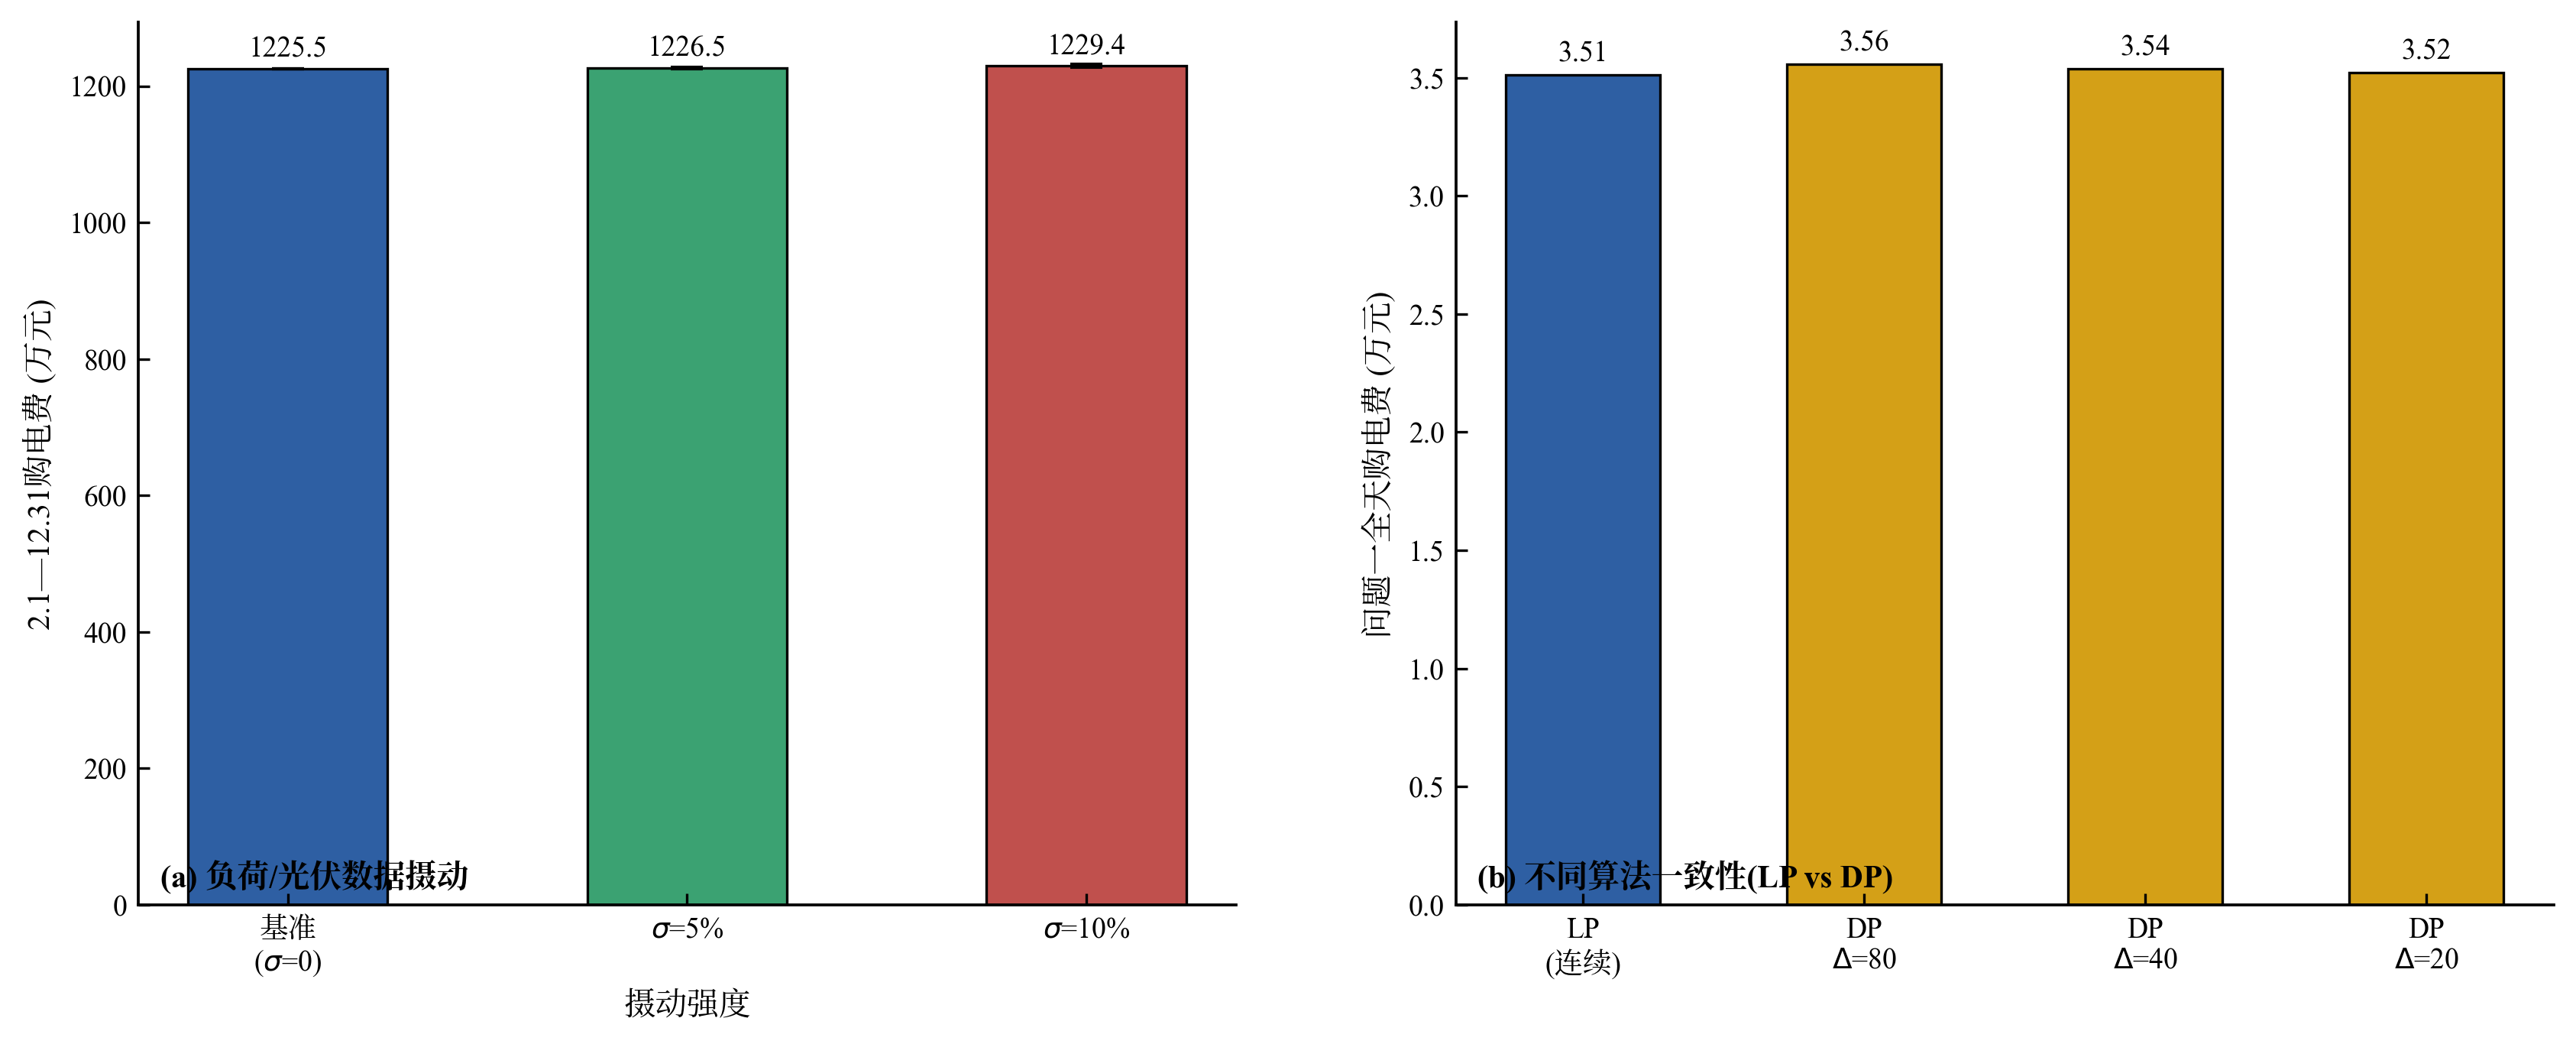
\includegraphics[width=0.88\textwidth]{求解/图片/图6-1_稳健性检验.png}
    \caption{稳健性检验：数据摄动与算法一致性对比}
    \label{fig:robust}
\end{figure}

\textbf{3.预报展开口径的敏感性}

5.3.2 节指出，附件三只给出每个预报时刻的整点预报值，将其展开到 10 分钟栅格存在多种口径。正文采用线性插值；作为对照，若改用“阶梯保持”口径（把每个整点预报值直接保持到下一个整点），在同一模型、同一费用公式下重新求解，2.1—12.31 的结果如表\ref{tab:expand}所示。

\begin{longtable}{>{\centering\arraybackslash}p{0.17\textwidth}>{\centering\arraybackslash}p{0.17\textwidth}>{\centering\arraybackslash}p{0.17\textwidth}>{\centering\arraybackslash}p{0.17\textwidth}>{\centering\arraybackslash}p{0.17\textwidth}}
  \caption{预报展开口径对结果的影响（2.1—12.31）}
  \label{tab:expand} \\
  \toprule
  展开口径 & 含调整总费用（元） & 无调整总费用（元） & 紧急购电量（kWh） & 紧急购电费（元） \\
  \midrule
  \endfirsthead
  \caption{预报展开口径对结果的影响（续）} \\
  \toprule
  展开口径 & 含调整总费用（元） & 无调整总费用（元） & 紧急购电量（kWh） & 紧急购电费（元） \\
  \midrule
  \endhead
  \bottomrule
  \endfoot
  线性插值（本文采用） & 14337999.15 & 14782072.51 & 416613.13 & 1713169.76 \\
  阶梯保持（对照） & 17948773.82 & 17884096.43 & 1223271.04 & 5391470.75 \\
\end{longtable}

{\emergencystretch=2em
表\ref{tab:expand}显示，两种口径给出的整点预报值完全相同，2.1—12.31 的总费用却相差 3610774.67 元。紧急购电量由 416613.13 kWh 变为 1223271.04 kWh，两者之比约为 $1:2.9$。在线性插值下引入滚动调整可节省 444073.36 元，而在阶梯保持下调整反而比不调整多支出 64677.39 元，结论发生反转。差别并不来自预报在整点处的精度：两口径的预报值在所有整点处逐点相同，全年逐时预报的平均绝对误差为 234.91 kW、均方根误差为 432.51 kW、平均偏差为 $+63.54$ kW，且各预报时刻在其 6 小时有效窗口内的分时段误差也完全一致（0:00、6:00、12:00、18:00 发布的预报对应的平均绝对误差分别为 $0$、$535.34$、$297.85$、$106.45$ kW）。真正的差别在于约束的时段归属：阶梯保持等价于额外假设“整点之间的出力保持不变”，该假设在附件二、附件三中均无依据，却把整点值强加给其后的每一个 10 分钟间隔，人为制造出 10 分钟尺度的瞬时供需缺口，进而放大紧急购电需求。\par}

据此，本文采用线性插值口径：它不改变任何整点处的预报取值，也不引入预报时刻之外的新信息，仅在相邻整点之间构造连续过渡，因而不具备系统性美化或恶化预报的机制。需要说明的是，这一结论只针对“整点值之间如何过渡”，不涉及预报本身的精度；附件三只给出整点值，10 分钟尺度的过渡方式无法由现有数据判定，本文将 3610774.67 元的量级差如实报告，以便在获得更细分辨率预报数据时复核。

\textbf{4.无储能对照}

为检验储能与滚动调整的实际价值，取消储能后重新求解同一模型（储电量恒为 0，全部用电均需从电网购入）：问题一全天购电费由 35126.95 元升至 48052.05 元，降幅 26.90\%；问题二 2.1—12.31 的总费用由 12254765.72 元升至 16407319.63 元，降幅 25.31\%。两个问题的改善幅度在同一量级，说明本文给出的经济性提升主要来自储能的削峰填谷，而非求解误差或口径选择。

\textbf{5.逐日收益的方向性}

总费用为累计量，会掩盖逐日差异。以“仅执行 0:00 计划”为基准逐日比较（2.1—12.31 共 334 天），有 155 天调整后的费用反而高于基准，最差的一天为 2025 年 9 月 29 日，多支出 9676.94 元；题目给出的四个代表日中，3 月 20 日节省 201.33 元，而 6 月 21 日、9 月 23 日、12 月 21 日分别多支出 764.72 元、3277.99 元与 707.19 元（逐日的计划与调整购电量见表\ref{tab:结果3-4}，全年逐日紧急购电量见图\ref{fig:结果3-3}）。原因是调整购电量与实际需求的偏差要按 1.5 倍惩罚计价，当预报误差方向与偏差方向不利时，调整反而增加支出，这与 5.3.4 节边际分析中“6:00 预报单独引入时边际收益为 $-3.74$ 万元”相互印证。全年累计仍净节省 444073.36 元，即 3.00\%，故滚动调整在期望意义上有效，但不宜宣称逐日均受益。

\textbf{6.适用边界}

（1）附件三仅给出整点预报值，其物理含义（瞬时值或小时平均值）题目未作说明。本文按瞬时值处理并对相邻整点作线性插值；若其实际含义为小时平均值，过渡段取值将发生改变，表\ref{tab:expand}已给出该不确定性对总费用的影响范围。（2）本文结论依赖“预报误差方向随机”这一隐含前提。逐日比较中出现的 155 天负收益说明，当预报出现系统性偏差（持续高估或低估）时，滚动调整的净节省会被侵蚀，甚至由正转负，此时应降低调整幅度或提高预报精度，而非单纯增加预报时刻；5.3.4 节的结果也表明，在有真实预报的前提下提高预报精度所能带来的收益远大于加密预报时刻。（3）模型未考虑电价的随机性与储能寿命成本，这两者会在长期运行中影响策略的经济性，可作为后续改进方向。
